
	\سؤال{مشاهده فراخوانی‌های سیستمی تعریف شده}

در این قسمت با توجه به این‌که ساختار سخت‌افزار ما با سوال فرق دارد، فایل \lr{asm} را به کمک دستور \lr{find} پیدا کردیم:

\begin{code}
	> cd /usr/include/
	
	> find . -name asm
	
	./x86_64-linux-gnu/asm
	
	> cd ./x86_64-linux-gnu/asm/
	
	> cat unistd.h
	
\end{code}

\begin{figure}[h!]
	\centering
	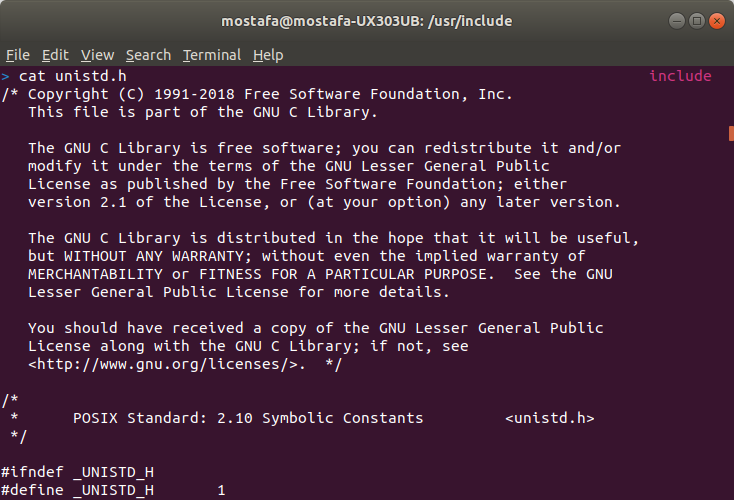
\includegraphics[scale=.4]{img/1.png}
\end{figure}

\سؤال{اجرای یک فراخوانی سیستمی}

\begin{itemize}
	\item 
	دستورات زیر را درون \lr{terminal} اجرا می‌کنیم.
	
	\begin{code}
		> mkdir 2 \&\& cd 2
		
		> sudo nano testsyscall.cpp
		
		
	\end{code}

	\item کد داده شده در سوال را در این قسمت کپی کرده و سپس با استفاده از دستور \lr{\lstinline{ctrl + x}} آن را ذخیره می‌کنیم.
	
	\item به کمک دستورات زیر کد را کامپایل کرده و اجرا می‌کنیم.
	
	\begin{code}
		> sudo gcc -o testsyscall testsyscall.cpp 
		
		> ./testsyscall
	\end{code}

	\item نتیجه‌ی اجرای آن ساخته شدن یک پوشه به نام \lr{testdir} در مسیر   \footnote{directory} فعلی است و در آخر پیام \lr{The result is 0.} را چاپ می‌کند.
	
	\item 
	همان‌طور که در توضیحات فراخوانی سیستمی آمده است، هر فراخوانی سیستم با یک شماره‌ی ثابت شناخته می‌شود. نقش \lr{\lstinline{\_\_NR\_mkdir}} (که به‌طور سراسری \footnote{global} تعریف شده است) در این‌جا این است تا عدد مربوط به این فراخوانی جایگرین آن شود.
	
	\begin{figure}[h!]
		\centering
		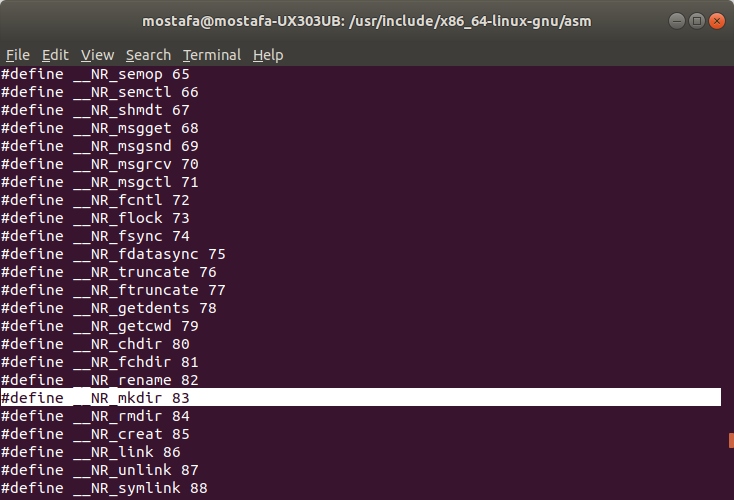
\includegraphics[scale=.4]{img/2.png}
	\end{figure}
	
	\item تابع \lr{\lstinline{syscall()}} یک تابع کوچک است که رابط زبان \lr{assembly} آن دارای شماره و آرگومان‌های مشخص است. تابع پر کاربردی است اگر از آن بدون \lr{wrapper}ها استفاده کنیم، رجسیترهای پردازنده قبل از فراخوانی سیستم ذخیره می‌کند و بعدا آن‌ها را بازگردانی می‌کند. خروجی آن در صورتی که با موفقیت انجام گیرد، «۰» و در غیر این صورت «۱-» خواهد بود.
\end{itemize}

\سؤال{اجرای ساده‌تر فراخوانی‌های سیستمی}
	
	\begin{Verbatim}[tabsize=4]
include <stdio.h>
include <unistd.h>
include <sys/stat.h>
int main() {
	long result;
	result = mkdir("testdir", 0777);
	printf("The result is %ld.\n", result);
	return 0;
}
	\end{Verbatim}